\section{Курсы}
\subsection{Роли и операции}

Раздел доступен пользователям, имеющим следующие роли:

\begin{itemize}
	\item Администратор вуза"=поставщика:
	\begin{itemize}
		\item возможность просматривать курсы в данном университете;
		\item возможность создания/редактирования курса в данном университете;
		\item возможность назначения авторов курса при создании/редактировании курса.
	\end{itemize}
	\item Администратор контента вуза"=поставщика:
	\begin{itemize}
		\item возможность просматривать курсы в данном университете;
		\item возможность редактирования курса в данном университете.
	\end{itemize}
	\item Автор курса:
	\begin{itemize}
		\item возможность просматривать свой курс;
		\item возможность редактировать свой курс;
		\item возможность назначать авторов своего курса.
	\end{itemize}
	\item Администратор Платформы:
	\begin{itemize}
		\item просматривать курсы любого университета;
		\item создавать курс в любом университете;
		\item редактирование любого курса;
		\item назначение команды курса.
	\end{itemize}
\end{itemize}
\subsection{Список курсов}
\label{course:subsec:course_list}
В данном разделе находится список курсов (рис.~\ref{img:course:course_list}).

\begin{figure}[H]
	\center{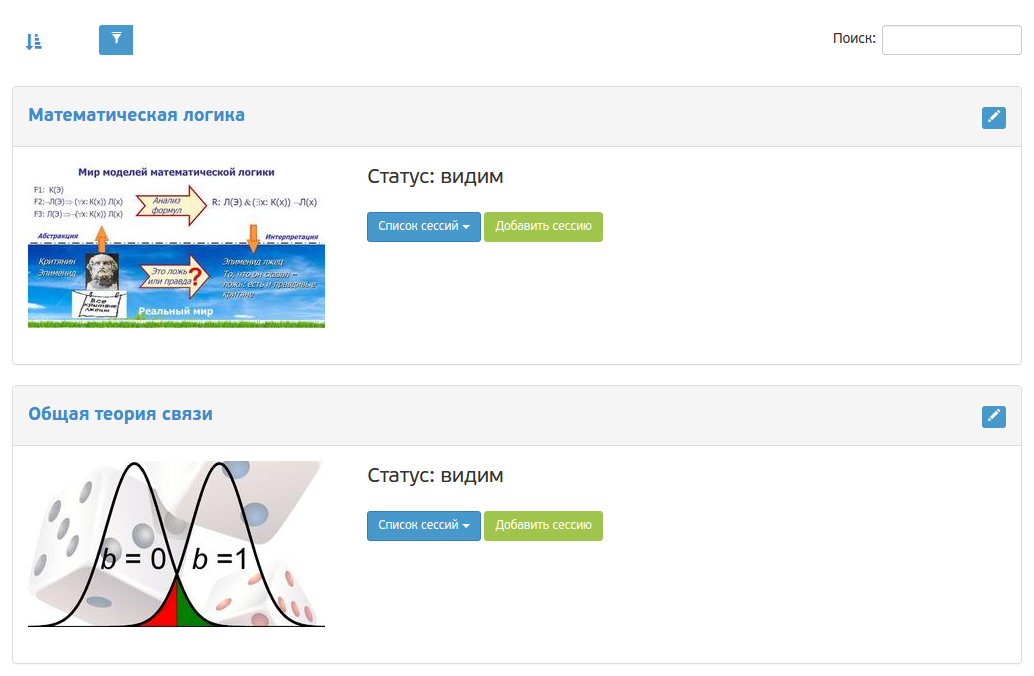
\includegraphics[width=1\linewidth]{images/course/course_list}}
	\caption{Внешний вид списка курсов.}
	\label{img:course:course_list}
\end{figure}

Каждый курс представлен отдельным элементом списка, на котором отображено:
\begin{itemize}
	\item Название курса. Если у пользователя есть право на просмотр данного курса, то при нажатии на название курса происходит переход на страницу подробной информации о курсе. Подробно форма детального просмотра курса описана в разделе~\ref{course:subsec:course_detail}).
	\item Если у пользователя есть право на редактирование данного курса, то пользователю доступна кнопка редактирования курса \vcenteredinclude[height=25px]{images/course/course_edit_btn}.
	\item Обложка курса.
	\item Статус курса (видим или скрыт).
	\item Если у курса есть сессии и пользователь имеет право на какое"=либо действие с сессиями данного курса, то ему доступна кнопка \quotes{список сессий}, при нажатии на которую пользователю становится доступна таблица со списком сессий данного курса (рис.~\ref{img:course:course_session_list}). При повторном нажатии на кнопку, таблица со списком сессий курса скрывается.
	\begin{figure}[H]
		\center{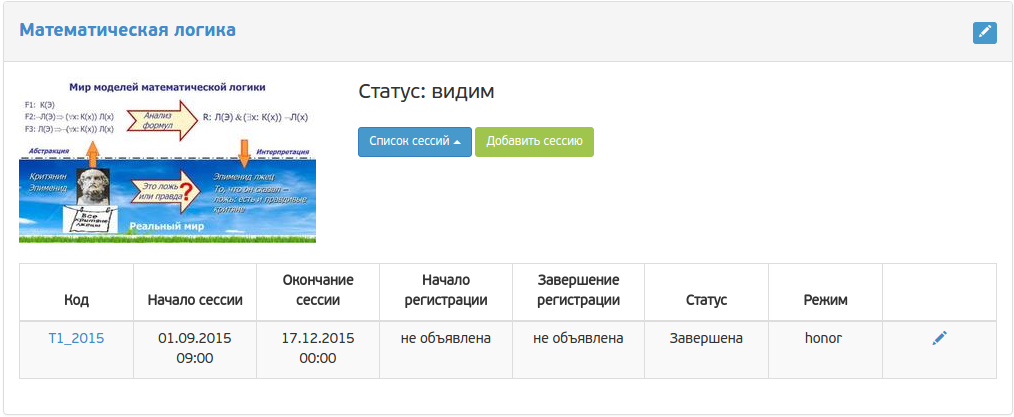
\includegraphics[width=1\linewidth]{images/course/course_session_list}}
		\caption{Список сессий курса}
		\label{img:course:course_session_list}
	\end{figure}
	
	\item Если у пользователя есть право на создание сессии, пользователю доступна кнопка \quotes{Добавить сессию}, при нажатии на которую пользователь переходит к окну создания сессии курса.
\end{itemize}

Единовременно на странице отображается не более 5 курсов. Если количество курсов больше пяти, происходит постраничное отображение курсов. Также на странице появляются элементы постраничной навигации (рис.~\ref{img:course:course_pagination}).

\begin{figure}[H]
	\center{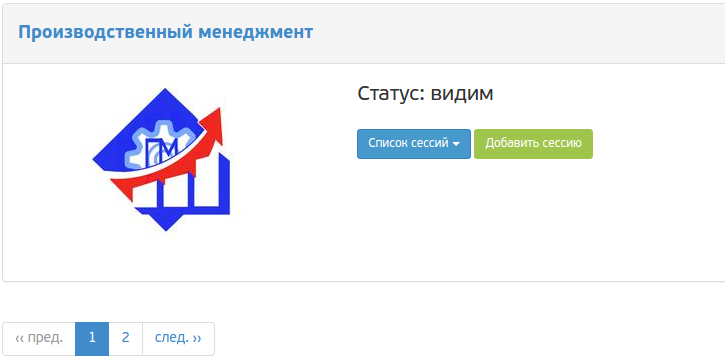
\includegraphics[width=1\linewidth]{images/course/course_pagination}}
	\caption{Элементы постраничной навигации при отображении курсов.}
	\label{img:course:course_pagination}
\end{figure}

Также имеется возможность упорядочить курсы в алфавитном порядке по возрастанию (убыванию) при помощи кнопки сортировки (рис.~\ref{img:course:course_filter_btn}).

\begin{figure}[H]
	\begin{minipage}[h]{0.49\linewidth}
		\center{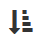
\includegraphics[width=0.1\linewidth]{images/course/course_sort_btn_az.png} \\ а)}
	\end{minipage}
	\hfill
	\begin{minipage}[h]{0.49\linewidth}
		\center{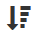
\includegraphics[width=0.1\linewidth]{images/course/course_sort_btn_za.png} \\ б)}
	\end{minipage}
	\caption{a) сортировка по возрастанию, б) сортировка по убыванию}
	\label{img:course:course_filter_btn}
\end{figure}

Также возможен поиск среди курсов данного вуза по имени и статусу путем ввода текста в поле поиска \vcenteredinclude[height=25px]{images/datatables/search} (рис.~\ref{img:course:course_filter}).

\begin{figure}[H]
	\center{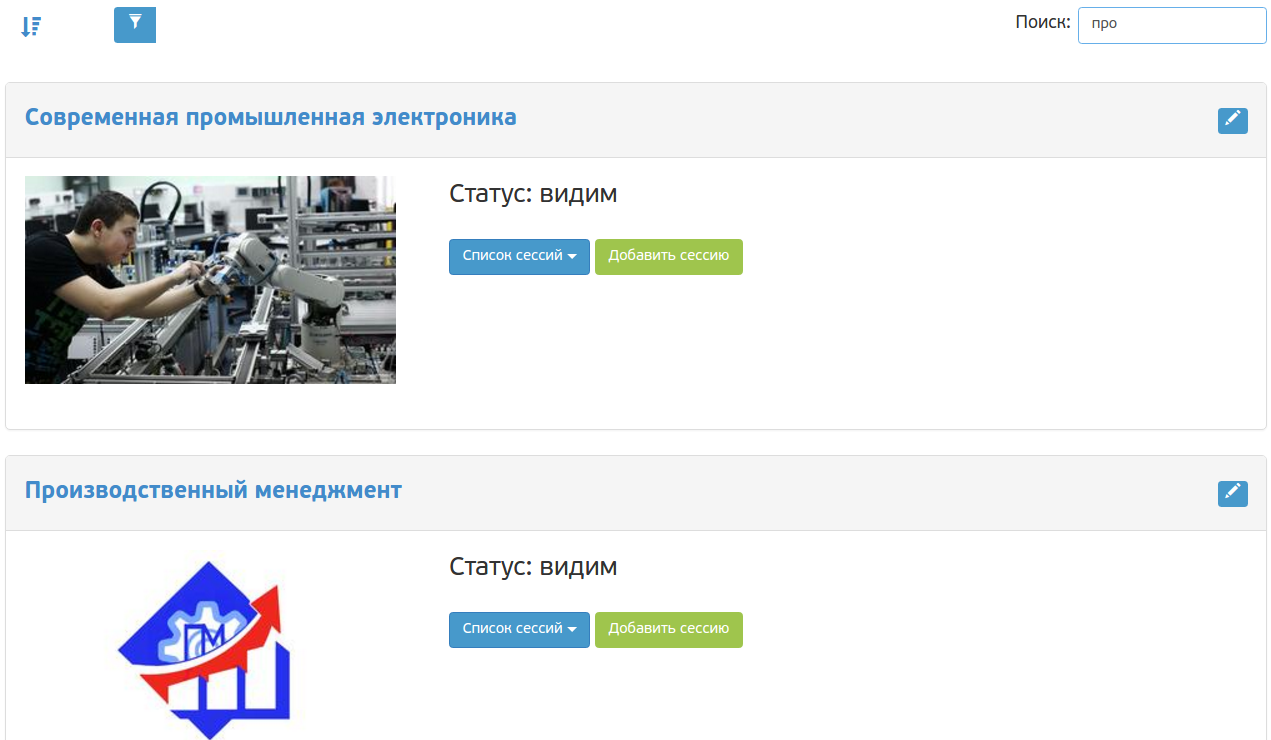
\includegraphics[width=1\linewidth]{images/course/course_filter}}
	\caption{Поиск курса по имени.}
	\label{img:course:course_filter}
\end{figure}

Возможна фильтрация курсов при помощи формы фильтрации, которая вызывается нажатием на кнопку фильтрации \vcenteredinclude[height=25px]{images/course/course_filter_form_btn}.

Форма фильтрации (рис.~\ref{img:course:course_filter_form}) позволяет фильтровать курсы по следующим параметрам:
\begin{itemize}
	\item название курса;
	\item статус курса (опубликован/скрыт);
	\item является ли данный курс рекомендованным (да/нет);
	\item находится ли данный курс в архиве (да/нет);
	\item преподаватель, который ведет курс (возможен выбор сразу нескольких см.\ раздел~\ref{widget:autocomplete_with_multiselect}).
\end{itemize}

\begin{figure}[H]
	\center{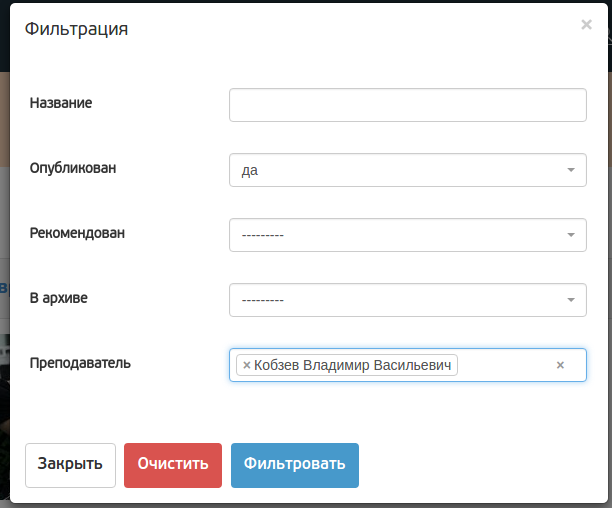
\includegraphics[width=1\linewidth]{images/course/course_filter_form}}
	\caption{Фильтр"=форма для списка курсов}
	\label{img:course:course_filter_form}
\end{figure}

При нажатии на кнопку \quotes{Фильтровать} происходит применение заданных пользователем фильтров. При нажатии на кнопку \quotes{Очистить} происходит очистка всех полей формы фильтрации. При нажатии на кнопку закрыть (или на крестик, или на область вне формы фильтрации), происходит закрытие формы фильтрации без применения фильтров.

Если применен хотя бы один фильтр, то рядом с кнопкой фильтрации появляется кнопка очистки формы фильтрации \vcenteredinclude[height=25px]{images/course/course_filter_form_btn_clear}.

Если у пользователя есть право на создание курса, то слева пользователю показывается кнопка
\vcenteredinclude[height=25px]{images/course/course_create_btn}, при нажатии на которую пользователь переходит на страницу создания курса.

Также, находясь в секции \quotes{Курсы}, пользователь в любой момент может перейти к списку курсов, нажав на кнопку \quotes{Список курсов}.

\subsection{Просмотра детальной информации о курсе}
\label{course:subsec:course_detail}
На данную страницу можно перейти, нажав на название курса на странице просмотра списка курсов, описанного в разделе~\ref{course:subsec:course_list}. Внешний вид страницы просмотра детальной информации о курсе представлен на рисунке~\ref{img:course:course_detail}.
\begin{figure}[H]
	\center{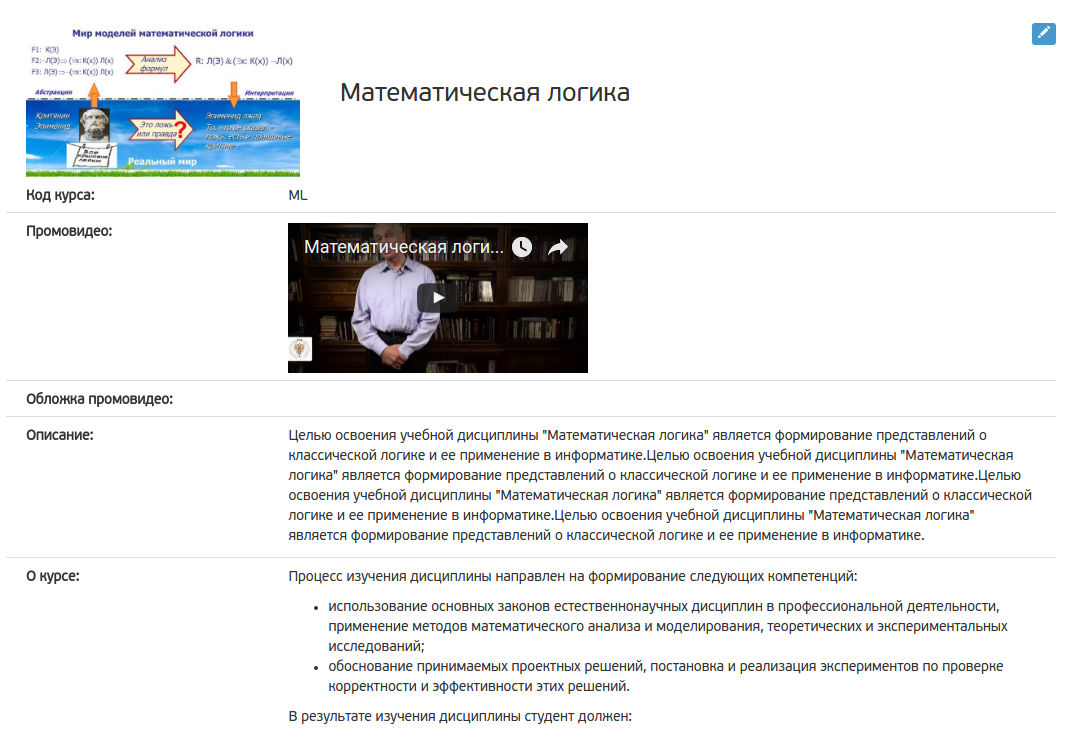
\includegraphics[width=1\linewidth]{images/course/course_detail}}
	\caption{Детальная информация о курсе}
	\label{img:course:course_detail}
\end{figure}

В верхней части данной страницы отображена обложка курса и его название. Если у пользователя есть право на редактирование данного курса, то в правом верхнем углу находится кнопка \vcenteredinclude[height=25px]{images/course/course_edit_btn}, нажатие на которую ведет к странице редактирования данного курса.

На странице отображается следующая информация о курсе:
\begin{itemize}
	\item обложка курса;
	\item название курса;
	\item код курса;
	\item промовидео;
	\item обложка промовидео;
	\item описание курса;
	\item о курсе;
	\item формат курса;
	\item ссылки на внешние ресурсы;
	\item результаты обучения;
	\item знания, навыки и умения, приобретаемые после прохождения курса;
	\item описание сертификата, который выдается по прохождении курса;
	\item значок сертификата;
	\item описание условий выдачи сертификата;
	\item компетенции образовательного стандарта;
	\item количество времени, которое нужно уделять для прохождения курса;
	\item количество зачетных единиц;
	\item опубликован ли данный курс;
	\item рекомендован ли данный курс;
	\item программа курса;
	\item требования к прохождению курса;
	\item дополнительная информация о курсе;
	\item дополнительная информация о курсе, которая будет размещена в правом блоке;
	\item список преподавателей, преподающих этот курс в порядке отображения на странице курса;
	\item список направлений подготовки, для которых предназначается этот курс;
	\item список групп дисциплин, для которых отображается данный курс;
	\item произвольные направления подготовки;
	\item список авторов курса.
\end{itemize}

\subsection{Создание/редактирование курса}
\label{course:subsec:course_create}
Форма создания/редактирования курса разбита на несколько блоков, для удобства заполнения:
\subsubsection{Основная информация}
	\begin{itemize}
		\item \textbf{Код курса} "--- уникальный (в рамках вуза) код курса. Должен иметь длину не более чем 25 символов, состоять из символов латинского алфавита верхнего и нижнего регистра. В случае, если курс с данным кодом существует в рамках данного университета, то внизу поля появится сообщение об ошибке (рис.~\ref{img:course:slug_error}). Обязательное поле. В режиме редактирования курса данное поле нельзя изменять.
		\begin{figure}[H]
			\center{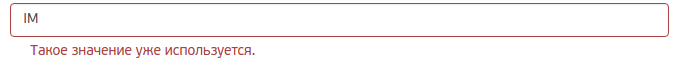
\includegraphics[width=1\linewidth]{images/course/slug_error}}
			\caption{Ошибка, указывающая на то, что курс с таким кодом уже существует}
			\label{img:course:slug_error}
		\end{figure}
		\item \textbf{Название} курса "--- может состоять из любых символов и иметь длину до 200 символов. Обязательное поле.
		\item \textbf{Университет} "--- название университета, к которому принадлежит курс. Нередактируемое поле.
		\item \textbf{Опубликован} "--- переключатель, задающий видимость данного курса на странице курсов, доступных для прохождения.
		\item \textbf{Рекомендован} "--- переключатель, задающий, является ли данный курс рекомендованным к прохождению.
		\item \textbf{Преподаватели} "--- список преподавателей, которые ведут данный курс. Для того, чтобы добавить нового преподавателя, необходимо нажать на кнопку \quotes{Добавить} (рис.~\ref{img:course:instructor_list}), после чего выбрать нужного преподавателя из списка (в списке содержатся только преподаватели из данного вуза). Также осуществляется фильтрация по ФИО преподавателя (подробнее в подразделе~\ref{widget:autocomplete}). Для того, чтобы убрать преподавателя из списка, необходимо нажать на \quotes{крестик} рядом с именем преподавателя. Порядок преподавателей можно изменять с помощью перетаскивания (подробнее в подразделе~\ref{widget:ordering}). Порядок преподавателей задает порядок отображения преподавателей на странице курса.
		\begin{figure}[H]
			\center{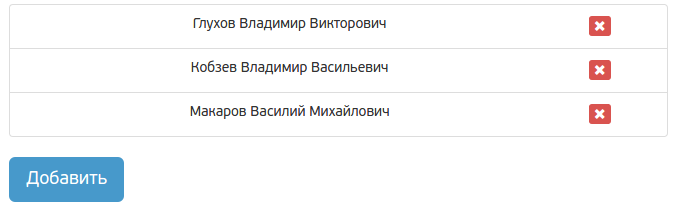
\includegraphics[width=1\linewidth]{images/course/instructor_list}}
			\caption{Поле для формирования списка преподавателей курса}
			\label{img:course:instructor_list}
		\end{figure}		

		\item \textbf{Группы дисциплин} "--- список дисциплин, для которых предназначается данный курс. Для того, чтобы добавить новую группу, необходимо нажать на кнопку \quotes{Добавить}, после чего выбрать нужную группу из списка. Также осуществляется фильтрация по названию группы (подробнее в пункте~\ref{widget:autocomplete}). Для того, чтобы убрать группу из списка, необходимо нажать на \quotes{крестик} рядом с названием группы.
		\item \textbf{Направления подготовки} "--- список направлений подготовки, для которых предназначается данный курс. Для того, чтобы добавить новое направление, необходимо нажать на кнопку \quotes{Добавить}, после чего выбрать нужное направление из списка. Также осуществляется фильтрация по названию направления подготовки (подробнее в пункте~\ref{widget:autocomplete}). Для того, чтобы убрать направление из списка, необходимо нажать на \quotes{крестик} рядом с названием группы.
		\item \textbf{Произвольные направления подготовки} "--- текстовое поле.
		\item \textbf{Авторы курса} "--- список авторов курса.  Для того, чтобы добавить нового пользователя в список авторов курса, необходимо нажать на кнопку \quotes{Добавить}, после чего выбрать нужного пользователя из списка. Также осуществляется фильтрация по имени пользователя и по адресу электронной почты (подробнее в пункте~\ref{widget:autocomplete}). Для того, чтобы убрать пользователя из списка, необходимо нажать на \quotes{крестик} рядом с именем преподавателя.
		\item \textbf{Список сессий курса} "--- список сессий данного курса, представленный в виде таблицы  (рис.~\ref{img:course:course_session_table}).
		\begin{figure}[H]
			\center{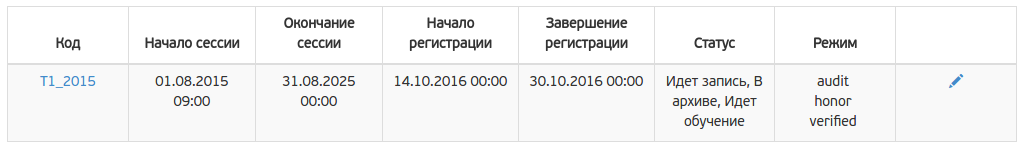
\includegraphics[width=1\linewidth]{images/course/course_session_table}}
			\caption{Таблица со списком сессий курса}
			\label{img:course:course_session_table}
		\end{figure}
		
		Таблица со списком сессий курса имеет следующие столбцы:
		\begin{itemize}
			\item \textbf{Код} "--- код сессии курса. При щелчке на код сессии, происходит переход на детальное отображение данной сессии курса (подробнее про отображение детальной информации о сессии курса описано в разделе~\ref{course_session:course_session_detail}.
			\item \textbf{Начало сессии} "--- дата начала сессии курса. В случае, если дата начала сессии курса не задана, отображается надпись \quotes{не объявлена}.
			\item \textbf{Окончание сессии} "--- дата окончания сессии курса. В случае, если дата окончания сессии курса не задана, отображается надпись \quotes{не объявлена}.
			\item \textbf{Начало регистрации} "--- дата начала регистрации на сессию курса. В случае, если дата начала регистрации не задана, отображается надпись \quotes{не объявлена}.
			\item \textbf{Завершение регистрации} "--- дата завершения регистрации на сессию курса. В случае, если дата завершения регистрации не задана, отображается надпись \quotes{не объявлена}.
			\item \textbf{Статус} "--- статус сессии курса.
			\item \textbf{Режим} "--- список возможных режимов прохождения сессии курса.
			\item Кнопка редактирования сессии курса \vcenteredinclude[height=25px]{images/course_session/session_edit_btn} "--- переводит пользователя на страницу редактирования данной сессии курса (отображается если у пользователя есть право на редактирование сессии курса).
		\end{itemize}
	\end{itemize}
\subsubsection{Дополнительная информация}
	\begin{itemize}
		\item \textbf{Описание} "--- текстовое поле, содержащее в себе краткое описание курса. Допускает HTML"=разметку (работа с данным полем описана в пункте~\ref{widget:ckeditor}).
		\item \textbf{О курсе} "--- текстовое поле, содержащее в себе описание курса.  Допускает HTML"=разметку (работа с данным полем описана в пункте~\ref{widget:ckeditor}). Если курс опубликован, то данное поле является обязательным и в нем должно быть записано не менее 200 значащих символов (символы латинского, русского алфавита, цифры и т.д.). В противном случае данное поле необязательно.
		\item \textbf{Формат курса} "--- текстовое поле, содержащее в себе описание формата курса. Допускает HTML"=разметку (работа с данным полем описана в пункте~\ref{widget:ckeditor}).
		\item \textbf{Внешние ресурсы} "--- текстовое поле, содержащее в себе ссылки на внешние ресурсы, которые могут помочь в освоении курса. Допускает HTML"=разметку (работа с данным полем описана в пункте~\ref{widget:ckeditor}).
		\item \textbf{Программа курса} "--- текстовое поле, содержащее в себе описание программы курса.Допускает HTML"=разметку (работа с данным полем описана в пункте~\ref{widget:ckeditor}).
		\item \textbf{Требования} "--- текстовое поле, содержащее в себе описание требований курса. Допускает HTML"=разметку (работа с данным полем описана в пункте~\ref{widget:ckeditor}).
		\item \textbf{Дополнительная информация} "--- текстовое поле, содержащее в себе дополнительную информацию о курсе. Допускает HTML"=разметку (работа с данным полем описана в пункте~\ref{widget:ckeditor}).
		\item \textbf{Дополнительная информация в правом блоке} "--- текстовое поле, содержащее в себе описание дополнительной информации, которая будет выводиться в правом блоке на странице просмотра курса. Допускает HTML"=разметку (работа с данным полем описана в пункте~\ref{widget:ckeditor}).
	\end{itemize}
\subsubsection{Результаты обучения}
	\begin{itemize}
		\item \textbf{Результаты обучения} "--- текстовое поле, содержащее в себе результаты прохождения курса. Допускает HTML"=разметку (работа с данным полем описана в пункте~\ref{widget:ckeditor}).
		\item \textbf{Знания} "--- текстовое поле, содержащее в себе описание знаний, которые человек получит в процессе прохождения курса. Допускает HTML"=разметку (работа с данным полем описана в пункте~\ref{widget:ckeditor}).
		\item \textbf{Навыки} "--- текстовое поле, содержащее в себе описание навыков, которые человек получит в процессе прохождения курса. Допускает HTML"=разметку (работа с данным полем описана в пункте~\ref{widget:ckeditor}).
		\item \textbf{Умения} "--- текстовое поле, содержащее в себе описание умений, которые человек получит в процессе прохождения курса. Допускает HTML"=разметку (работа с данным полем описана в пункте~\ref{widget:ckeditor}).
	\end{itemize}
\subsubsection{Нагрузка}
	\begin{itemize}
		\item \textbf{Часов в неделю от} "--- минимальная нагрузка в неделю. Может принимать значение от 1 до 40. Если указана максимальная нагрузка, то необходимо указать минимальную, при этом минимальная нагрузка не должна быть больше максимальной.
		\item \textbf{Часов в неделю до} "--- максимальная нагрузка в неделю. Может принимать значение от 1 до 40. Если указана минимальная нагрузка, то необходимо указать максимальную, при этом максимальная нагрузка не должна быть меньше минимальной.
		\item \textbf{Зачётных единиц} "--- количество зачетных единиц, которые необходимо сдать для успешного завершения курса. Может принимать значение от 1 до 10.
		\item \textbf{Длительность (недель)} "--- продолжительность (в неделях) курса. Может принимать значение от 1 до 16.
	\end{itemize}
\subsubsection{Медиа}
	\begin{itemize}
		\item \textbf{Обложка} "--- обложка курса, отображаемая пользователю. Ширина и высота загружаемого изображения не должны превышать 600 пикселей, а размер изображения не должен быть больше 1 Мб.
		Возможно загружать изображения в следующих форматах: png, jpg, jpeg, gif. Процесс загрузки изображения описан в пункте~\ref{widget:file_upload}.
		\item \textbf{Промовидео} "--- ссылка на промовидео курса.
		\item \textbf{Картинка для видео} "--- обложка для промовидео. Ширина и высота загружаемого изображения не должны превышать 600 пикселей, а размер изображения не должен быть больше 1 Мб. Возможно загружать изображения в следующих форматах: png, jpg, jpeg, gif. Процесс загрузки изображения описан в пункте~\ref{widget:file_upload}.
	\end{itemize}
\subsubsection{Информация о сертификате}
	\begin{itemize}
		\item \textbf{Сертификат} "--- текстовое поле, содержащее в себе описание выдаваемого сертификата, которые человек получит после прохождения курса. Допускает HTML"=разметку  (работа с данным полем описана в пункте~\ref{widget:ckeditor}).
		\item \textbf{Компетенции образовательного стандарта} "--- текстовое поле, содержащее в себе описание компетенции образовательного стандарта. Допускает HTML"=разметку (работа с данным полем описана в пункте~\ref{widget:ckeditor}).
		\item \textbf{Значок сертификата} "--- обложка для промовидео. Ширина и высота загружаемого изображения не должны превышать 600 пикселей, а размер изображения не должен быть больше 1 Мб. Возможно загружать изображения в следующих форматах: png, jpg, jpeg, gif. Процесс загрузки изображения описан в пункте~\ref{widget:file_upload}.
		\item \textbf{Описание условий выдачи сертификата} "--- текстовое поле, содержащее в себе описание условий выдачи сертификата о прохождении курса. Допускает HTML"=разметку (работа с данным полем описана в пункте~\ref{widget:ckeditor}).
	\end{itemize}
\subsubsection{Элементы управления}
	\begin{itemize}
		\item \vcenteredinclude[height=25px]{images/course/form_cancel_btn} "--- кнопка отмены сохранения формы. При нажатии на данную кнопку пользователь будет перенаправлен предыдущую страницу.
		\item \vcenteredinclude[height=25px]{images/course/form_view_btn} "--- кнопка предпросмотра курса. При нажатии на данную кнопку пользователю будет показано, как курс будет отображаться пользователям. Закрытие модального окна производится нажатием на крестик в верхнем правом углу окна или щелчком за пределами данного окна.
		\begin{figure}[H]
			\center{
\includegraphics[width=1\linewidth]{images/course/course_preview}}
			\caption{Пример предпросмотра курса}
			\label{img:course:course_preview}
		\end{figure}
		
		\item \vcenteredinclude[height=25px]{images/course/form_save_btn} "--- кнопка сохранения курса. Если параметры курса заданы корректно, то при нажатии на кнопку будет произведено сохранение курса, а пользователь будет перенаправлен на страницу списка курсов. В противном случае будет произведена прокрутка до первого поля, в котором обнаружена ошибка.
	\end{itemize}